\chapter{基于RNN的深度强化学习混合模型在直复营销场景中的建模}
% 首先介绍直复营销问题使用强化学习研究的现状(函数逼近存在的问题,以及现行的解决方案和思路,从而引出本文的方法思路)
% 介绍深度强化学习
% 介绍本文提出的混合网络模型算法
在直复营销的场景中,企业以追求客户的生命周期价值最大化为目标,这与强化学习以追求累计奖赏最大的目标不谋而合。另外,在该场景中企业需要与顾客不断的进行营销行为,因此属于序列决策问题,并且因为场景的复杂性,还存在用户状态部分可观测的问题。而以RNN为代表的循环神经网络正巧可以在很好的处理序列问题的基础上,还可以利用神经网络自动的学习隐藏状态的表达方式。所以,结合以上两点,本章提出了基于RNN的深度强化学习的混合模型。在该模型中,使用RNN网络来学习和提高针对隐藏状态的表征能力,然后利用DQN网络来逼近Q值函数,充分利用了两个模型的优点。另外,为了提高训练时收敛的速度和精度,提出了两种改进的混合模型网络:一步混合模型1-RNN+DQN和两步混合模型2-RNN+DQN。

\section{直复营销问题概述}
直复营销是客户关系管理中的一项重要议题。它是通过企业长时间的与客户进行营销交互,并且结合所采取的营销行为和客户的响应情况进行分析,
以此来判断客户的对营销产品的喜好,进而可以辅助企业进行之后的营销决策。具体来说,在每个需要进行营销的时刻点,企业会对客户采取营销行为,比如发送宣传单、促销邮件或者优惠券等等,作为反馈,客户可能会访问该企业的相关资讯或者会完成一定金额的订单又或者会简单的忽略掉此次的营销行为。所以,企业需要在进行营销活动的时候做出对哪些客户进行营销的决策,以使的企业产生的收益最大化。

在直复营销场景中,我们需要注意的是,假如企业在某一时刻对某一客户采取了营销行为,客户可能会即刻给出反馈,也能会过了很长时间才会产生反馈信息。也就是说,营销行为对用户的影响是长期的而且用户对营销行为的反应是存在延迟的。所以,企业通常把最大化用户生命周期价值(Life-Time Value, LTV)作为评价营销效果的重要指标\citep{dwyer1997customer}。通过前面的介绍,我们知道强化学习在学习过程中考虑了延迟奖赏,并且以追求长期回报最大化为目标,所以直复营销问题就可以自然的表述为一个基本的强化学习问题,其中,即时利润看作是奖赏,LTV作为长期的价值函数。文献\citep{tkachenko2015autonomous,pednault2002sequential,silver2013concurrent}都正是以此想法为出发点,将强化学习技术应用在广告营销中,并且取得了较好的表现。

然而,与机器人和人机交互等现实应用场景中所面临的问题类似,在直复营销场景中,客户的状态(马尔科夫状态)是部分可观测的,这影响了强化学习技术在这些场景中的表现。根据马尔科夫性我们可以知道,客户的当前状态可以完全概括了他与企业在此之前的整个交互历史,也就是说客户的未来响应情况与之前的交互历史无关,只与在当前状态和未来的行为有关。然而,在直复营销这种复杂的现实场景中,构建这种具有马尔科夫性的状态是很难的。即使像在直复营销中比较常用的Recency-Frequency-Monetary用户价值模型\citep{tkachenko2015autonomous},也仅仅捕获到了客户真实状态中的部分信息。因此,对这些场景使用强化学习之前,进行隐藏状态的推断表示是很重要的。

在强化学习的研究和应用中,处理部分可观测状态最常用的方法就是使用部分可观测的马尔科夫决策过程(Partially Observable Markov  Decision Process,POMDP)\citep{kaelbling1998planning},并且已经在一些诸如机器人、人机对话等领域取得了不错的表现\citep{pineau2003point,williams2007partially}。在POMDP中,因为agent对环境观测的局限性,所以多了一步agent对当前所处状态可信度的判断,
但是对当前状态可信度的判断需要借助领域专家自定义的隐状态,而这些领域知识在一些复杂的现实应用中是很难获得的。

近年来,深度强化学习成功的应用在了游戏、围棋等领域。它们主要是将强化学习技术和深度神经网络相结合,其中,利用神经网络在逼近价值函数的同时也可以推断出环境的隐含状态表示方法。与POMDP不同的是,深度神经网络在不依靠专家领域知识的前提下,对任何给定的问题都可以自动的给出隐藏状态的合理表示方法\citep{deng2014deep},从而解决了在设计隐状态时所面临的困扰。以上本文选择使用深度强化学习解决直复营销问题的出发点,特别的,我们对现有的网络结构做了近一步的改进优化。

\section{深度强化学习DQN}
\subsection{Q-learning回顾}
在算法$\ref{algo:algorithm_2}$中,我们对Q-learning算法做了详细介绍,Q-learning方法主要思想是异策略的时间差分方法。

异策略,就是指的行为策略(产生数据的策略)和要评估的策略不是一个策略。在Q-learning中,行为策略是第6行的$\epsilon-greedy$的策略,而用于评估和改善的策略是第7行的贪婪策略(每个状态取值函数最大的那个行为)。

时间差分方法,是指利用时间差分目标来更新当前行为的值函数。在Q-learning中,时间差分的目标就是$r+\gamma \max_{a} Q(s^{'},a^{'})$。
\subsection{DQN}
 深度强化学习以DQN最为代表性,它就是在Q-learning的基础上修改得到的,主要进行了以下三个方面的改进。

 \paragraph{利用卷积神经网络逼近值函数}
 DQN利用深度卷积神经网络逼近值函数。如图\ref{fig:CNN_DQN}所示为状态行为值函数的逼近网络结构。利用神经网络逼近值函数属于参数化的非线性逼近方法,不仅具有很强的表征能力,而且还可以自动的捕捉到环境的隐状态信息。此处的值函数对应着一组参数,也就是神经网络中每层网络的参数,我们可以用向量$\mathbf{\theta}$表示,对应的值函数可以表示为$Q(s,a;\mathbf{\theta})$,所以对值函数的更新也就是对参数向量$\mathbf{\theta}$,当网络结构确定后,$\mathbf{\theta}$就代表着值函数。DQN所使用的网络结构是三个卷基层加两个全连接层。
\begin{figure}[htbp]
\centering
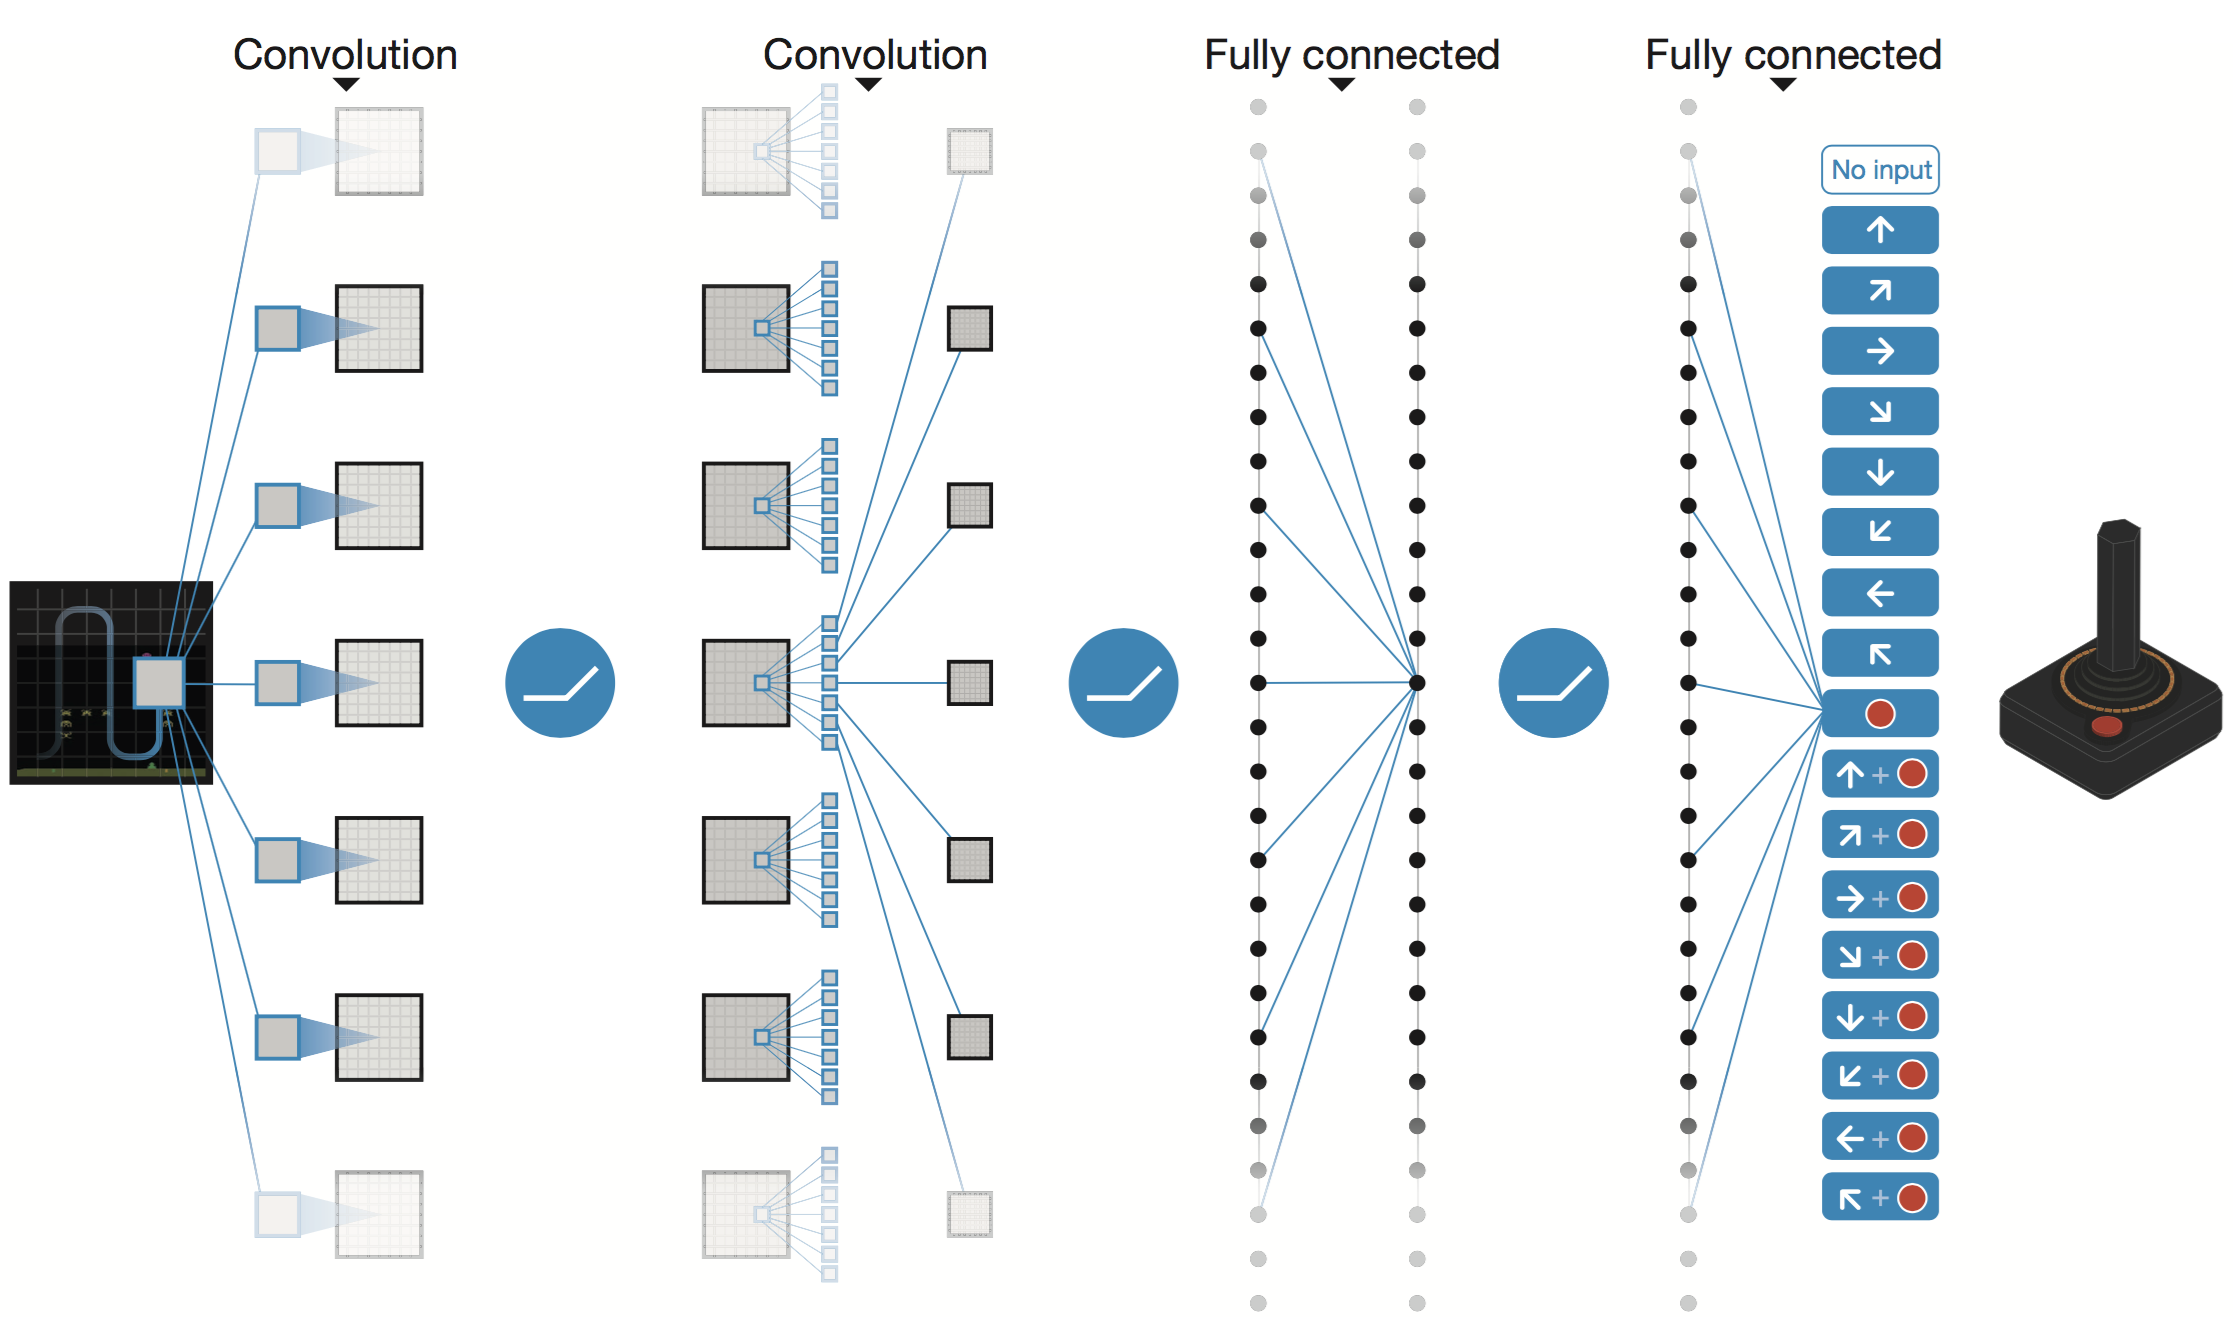
\includegraphics[width=1.0\textwidth]{CNN_DQN}
\caption{DQN状态行为值函数逼近网络}
\label{fig:CNN_DQN}
\end{figure}

其实,1995年Bertsekas等人最早将神经网络应用在在强化学习的值函数逼近中,取得了相比线性逼近较好的结果,但是往往会出现不稳定不收敛的情况\citep{bertsekas1995neuro}。此后,众多学者在这个方向上一直没有突破,直到DeepMind团队的出现。

 \paragraph{设置经验回放机制}
DeepMind团队的创始人Hassabis是神经科学的博士,他主要研究人类大脑中的海马体,海马体是大脑中主要负责记忆和学习的部分。他在研究时发现,人类在睡觉的时候,海马体会把一天的记忆重放给大脑皮层,利用这个启发机制,DeepMind团队的研究人员设计了一种神经网络的训练方法:经验回放。

经验回放是指,在强化学习的过程中,agent将数据存储在一个数据库中,再利用均匀采样的方法从数据库中抽取数据,然后利用抽取的数据训练神经网络。通过这种方法可以使的神经网络训练收敛且稳定。因为在训练神经网络时,我们假设的前提是训练数据是独立同分不的,但是通过强化学习采集的数据之间存在关联性,利用这些数据进行顺序训练,神经网络难免会不稳定。但是利用经验回放可以打破这种数据间的关联性。

 \paragraph{设置独立的目标网络}
与表格型Q-learning强化学习算法不同的是,利用神经网络对值函数进行逼近时,对值函数的更新其实就是对参数向量$\mathbf{\theta}$的更新,其更新方法时梯度下降法,因此算法$\ref{algo:algorithm_2}$第7行值函数的更新实际上变成了进度学习的一次更新过程,其梯度下降法为:
\begin{displaymath}
\begin{aligned}
\mathbf{\theta}_{t+1}=\mathbf{\theta}_{t}+\alpha[r+\gamma \max_{s^{'}}Q(s^{'},a^{'};\mathbf{\theta})-Q(s,a;\mathbf{\theta})]\triangledown Q(s,a;\mathbf{\theta})
\end{aligned}
\end{displaymath}
其中,$r+\gamma \max_{s^{'}}Q(s^{'},a^{'};\mathbf{\theta}$为TD目标,在计算$\max_{s^{'}}Q(s^{'},a^{'};\mathbf{\theta}$时用到的参数向量为$\mathbf{\theta}$。

我们称计算TD目标时所用的网络为TD网络。在DQN算法出现之前,利用神经网络逼近值函数时,计算TD目标的状态行为值函数所用的网络参数$\mathbf{\theta}$,与梯度计算中要逼近的值函数所用的网路参数向量相同,这样就容易导致数据间存在关联性,从而使训练不稳定。为了解决此问题,DeepMind提出计算TD目标的网络参数为$\mathbf{\theta}^{-}$,计算值函数逼近网络表示为$\mathbf{\theta}$;用于状态行为值函数逼近的网络每一步都要更新,而用于计算目标的网络则是每个固定的步骤更新一次。

因此,值函数的更新变为:
\begin{displaymath}
\begin{aligned}
\mathbf{\theta}_{t+1}=\mathbf{\theta}_{t}+\alpha[r+\gamma \max_{s^{'}}Q(s^{'},a^{'};\mathbf{\theta^{-}})-Q(s,a;\mathbf{\theta})]\triangledown Q(s,a;\mathbf{\theta})
\end{aligned}
\end{displaymath}

 \paragraph{DQN框架}
 由此,结合Q-learning算法并经过以上三个方面的改进,我们可以得到DQN的算法流程图$\ref{fig:liuchengtu_DQN}$:
\begin{figure}[htbp]
\centering
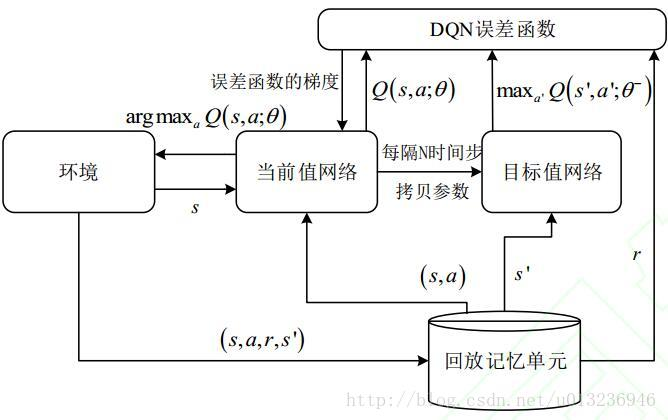
\includegraphics[width=0.9\textwidth]{liuchengtu_DQN}
\caption{DQN流程图}
\label{fig:liuchengtu_DQN}
\end{figure}

从图中,我们可以看出,DQN的主要学习过程包括以下几步:

(1)构建回放记忆单元。在每个情节中,初始化第一个状态$s$,并在接下里的每个时间点,按照$\epsilon-greedy$选择行为$a$,然后在仿真器中执行,可以得到即时奖赏$r$,下一步的状态$s^{'}$。并将此转换样本($s,a,r,s^{'}$)放到回放构建单元中。

(2)值函数的学习。从回报记忆单元中随机选取一条转移记录($s,a,r,s^{'}$),并分别使用当前值网络和目标值网络分别计算出值函数的估计值 $Q(s,a;\mathbf{\theta})$和TD目标值$r+\gamma \max_{s^{'}}Q(s^{'},a^{'};\mathbf{\theta^{-}})$,然后求出损失函数$L=(r+\gamma \max_{s^{'}}Q(s^{'},a^{'};\mathbf{\theta^{-}})-Q(s,a;\mathbf{\theta}))^{2}$,并使用梯度下降法进行求解。具体的损失函数参见图$\ref{fig:liuchengtu_DQN}$

(3)更新目标网络参数。经过若干步的训练后,将估计网络的参数拷贝给目标网络参数。

\begin{figure}[htbp]
\centering
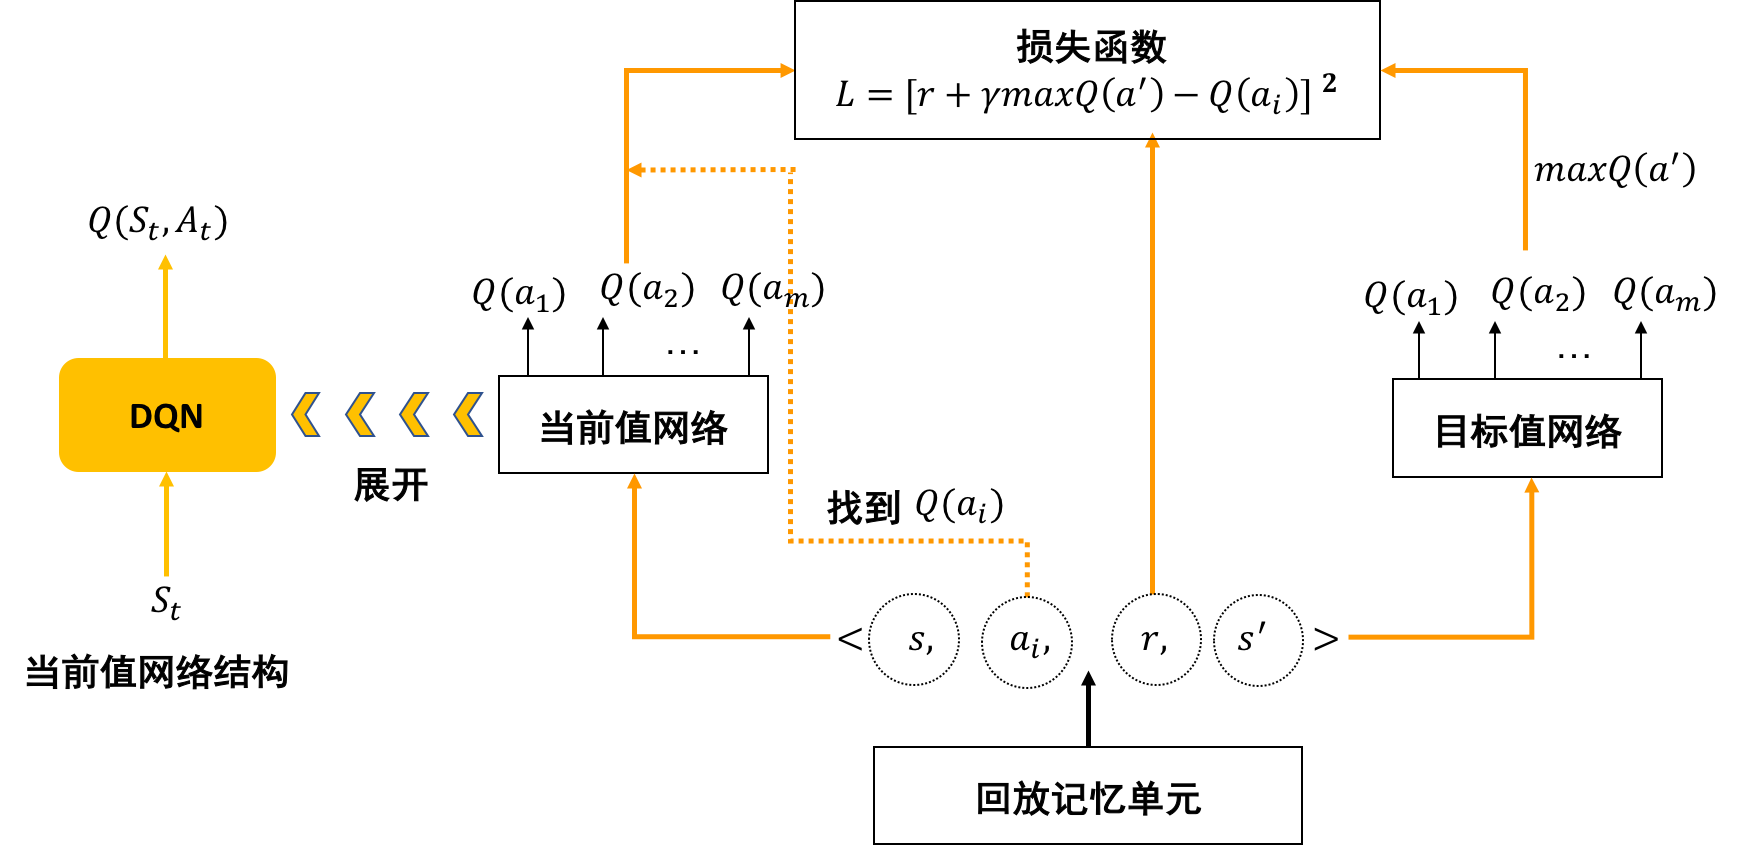
\includegraphics[width=0.8\textwidth]{loss_DQN}
\caption{DQN损失函数构造}
\label{fig:loss_DQN}
\end{figure}

结合算法$\ref{algo:algorithm_2}$,我们可以得出DQN算法的具体过程,其伪代码如算法$\ref{algo:algorithm_DQN}$所示。
\begin{algorithm}[htbp]
\small
\SetAlgoLined
\SetKwRepeat{Repeat}{repeat}{until} 
初始化回放记忆库$D$,记忆库大小为$N$\;
利用随机权值$\mathbf{\theta}$初始化状态行为值函数$Q$\;
初始化$\mathbf{\theta}^{-}$令$\mathbf{\theta}^{-}=\mathbf{\theta}$,用以计算TD目标的状态行为值$\hat{Q}$\;
\For{$episode=1,\cdots, M$}{
	初始化情节的第一个状态:$s_{1}={x_{1}}$(${x_{1}}$为环境的观测特征),通过预处理得到状态对应的特征输入:$\phi_{1}=\phi(s_{1})$\;
	\For{$t=1,\cdots, T$}{
		以概率$\epsilon$选一个随机行为$a_{t}$\;
		如果以上小概率事件没有发生,则按照贪婪策略选择当前值函数最大的那个行为:$a_{t}=\argmax_{a}Q(\phi(s_{t}),a;\mathbf{\theta})$\;
		在仿真器中执行行为$a_{t}$,可以观测到奖赏$r_{t}$以及下一步的环境的观测特征\;
		设置$s_{t+1}=s_{t},a_{t},x_{t+1}$,预处理得到对应的特征输入:$\phi_{t+1}=\phi(s_{t+1})$\;
		将转换样本($\phi_{t}, a_{t}, r_{t}, \phi(s_{t+1})$)放到回放记忆库中\;
		从回放记忆库D中均匀随机采样一个转换样本数据($\phi_{j}, a_{j}, r_{j}, \phi(s_{j+1})$)\;
		判断是否是一个情节的终止状态,若是,则TD目标位$r_{j}$,否则利用TD目标网络$\mathbf{\theta}^{-}$计算TD目标$r+\gamma \max_{s^{'}}Q(s^{'},a^{'};\mathbf{\theta^{-}})$\;
		执行一次梯度下降算法:$\triangle \theta = \alpha [r+\lambda \max_{a^{'}}Q(s^{'},a^{'};\theta^{-})-Q(s,a;\theta) ]\triangledown_{Q}(s,a;\mathbf{\theta})$\;
		更新状态行为值函数逼近的网络参数:$\mathbf{\theta}=\mathbf{\theta}+\triangle \theta$\;
		每隔$C$步更新一次TD目标网络权值;即:$\mathbf{\theta}^{-}=\mathbf{\theta}$\;
	}
}
% 输出最终策略:$\pi(s)=\argmax_{a}Q(s,a)$\;
\caption{DQN伪代码}
\label{algo:algorithm_DQN}
\end{algorithm}


\section{基于LSTM的深度强化学习混合模型设计}
\subsection{RNN和LSTM}
在DQN中,值函数逼近所使用的是卷积神经网络,它的结构有一个特点:就是假设输入是一个独立的没有上下文联系的单位。但是在序列化问题中,前面的输入和后面的输入是有关系的,也就是要具有针对长时间信息的记忆功能。所以,我们考虑使用循环神经网络(recurrent neural networks,RNN)和它的改进版本长短时记忆网络(ong short-term memory,lstm)来学习强化学习中状态的表示。因为循环网络的模型可以聚合过去的部分信息,并且可以捕捉到序列的长短时依赖性。因此,在处理序列问题上,它们的表现要优于卷及神经网络的性能。
 \paragraph{RNN}
RNN(Recurrent Neuron Network)是一种对序列数据建模的神经网络,即一个序列当前的输出与前面的输出也有关。具体的表现形式为网络会对前面的信息进行记忆并应用于当前输出的计算中,即隐藏层之间的节点不再无连接而是有连接的,并且隐藏层的输入不仅包括输入层的输出还包括上一时刻隐藏层的输出。图$\ref{fig:rnn}$是一个RNN模型的示例图。
\begin{figure}[htbp]
\centering
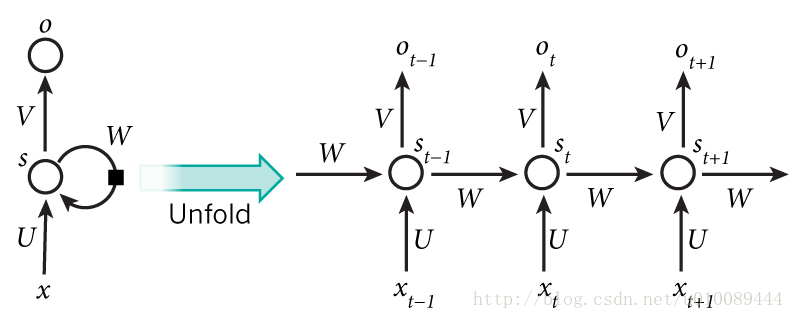
\includegraphics[width=0.8\textwidth]{rnn}
\caption{rnn模型}
\label{fig:rnn}
\end{figure}

在图$\ref{fig:rnn}$中:$x_{t}$表示$t$时刻的输入。$s_{t}$是$t$时刻的隐状态(memory),基于上一时刻的隐状态和当前输入得到:$s_t=f(U x_{t}+W s_{t−1})$,其中$f$一般是非线性的激活函数,在计算$s_{0}$时,即第一个单词的隐藏层状态,需要用到$s_{−1}$,但是其并不存在,在实现中一般置为0。$o_{t}$表示$t$时刻的输出。$\mathbf{U}$是输入层到隐藏层的权重矩阵,$\mathbf{V}$是隐藏层到输出层的权重矩阵,权重矩阵$\mathbf{W}$就是隐藏层上一次的值作为这一次的输入的权重。需要注意的是:在传统神经网络中,每一个网络层的参数是不共享的。而在RNN中,所有层次均共享同样的参数(例如上例中的$\mathbf{U}$,$\mathbf{V}$,$\mathbf{W}$)。其反应出RNN中的每一步都在做相同的事,只是输入不同,因此大大地降低了网络中需要学习的参数。

这个网络在$t$时刻接收到输入$x_{t}$之后,隐藏层的值是$s_{t}$,输出值是$o_{t}$。特别的,$o_{t}$的值不仅仅取决于$x_{t}$,还取决于$o_{t-1}$。我们可以用下面的公式来表示循环神经网络的计算方法:
\begin{equation}
\label{rnn_1}
\begin{aligned}
o_{t}=g(\mathbf{V}s_{t})
\end{aligned}
\end{equation}
\begin{equation}
\label{rnn_2}
\begin{aligned}
s_{t}=f(\mathbf{U}x_{t}+\mathbf{W}s_{t-1})
\end{aligned}
\end{equation}
式\eqref{rnn_1}是输出层的计算公式,输出层是一个全连接层,也就是它的每个节点都和隐藏层的每个节点相连。$\mathbf{V}$是输出层的权重矩阵,$g$是激活函数。式\eqref{rnn_2}是隐藏层的计算公式,它是循环层。$\mathbf{U}$是输入$x$的权重矩阵,$\mathbf{W}$是上一次的值作为这一次的输入的权重矩阵,$f$是激活函数。

从上面的公式我们可以看出,循环层和全连接层的区别就是循环层多了一个权重矩阵$\mathbf{W}$。

如果反复把式$\eqref{rnn_2}$带入到式$\eqref{rnn_1}$,我们将得到:
\begin{equation}
\begin{aligned}
o_{t}&=g(\mathbf{V}s_{t})\\
&=\mathbf{V}f(\mathbf{U} x_{t}+\mathbf{W} s_{t-1})\\
&=\mathbf{V}f(\mathbf{U} x_{t}+\mathbf{W} f(\mathbf{U} x_{t-1}+\mathbf{W} s_{t-2}))\\
&=\mathbf{V}f(\mathbf{U} x_{t}+\mathbf{W} f(\mathbf{U} x_{t-1}+\mathbf{W} f(\mathbf{U} x_{t-2}+\mathbf{W} f(\mathbf{U} x_{t-3}+\cdots)))\\
\end{aligned}
\end{equation}

从上面可以看出,循环神经网络的输出值$o_{t}$,是受前面历次输入值$x_{t}$、$x_{t-1}$、$x_{t-2}$、$x_{t-3}$、$\cdots$影响的,这就是为什么循环神经网络可以往前看任意多个输入值的原因。

循环神经网络的训练方法可以采用基于时间的反向传播算法(Backpropagation through time, BPTT),具体的更新方法和BP更新方法相同。但是,在处理较长序列的时候,普通循环神经网络不能得到较好的性能。一个主要原因是,RNN在训练中如果向前考虑的很远的时候,会导致对应的误差项的值增长或者缩小的非常快,就会很容易发生梯度爆照或者梯度消失的现象,这导致训练时梯度不能在较长序列中一直传递下去,从而使RNN无法捕捉到长距离的影响。

通常来说,梯度爆炸更容易处理一些。因为梯度爆炸的时候,我们的程序会收到NaN错误。我们也可以设置一个梯度阈值,当梯度超过这个阈值的时候可以直接截取。梯度消失更难检测,而且也更难处理一些,除了合理的初始化权重值、使用relu代替sigmoid和tanh作为激活函数外,还可以使用其他诸如长短时记忆网络(LTSM)的方法。其中后者是目前最流行的方法。

 \paragraph{LSTM}
原始RNN的隐藏层只有一个状态,它对于短期的输入非常敏感,LSTM在此基础上增加了一个状态,让它保存长期的状态。从而解决了传统RNN无法处理长距离依赖的问题。新增加的状态称为单元状态(cell state)。

如图$\ref{fig:lstm_2}$所示为lstm的展开结构,灰色矩形部分是一个lstm的简化结构,其中h为原始RNN的隐藏层状态,c为单元状态。从图中我们可以看出,在t时刻,LSTM的输入有三个:当前时刻网络的输入值$x_{t}$、上一时刻LSTM的输出值$h_{t-1}$、以及上一时刻的单元状态$c_{t-1}$;LSTM的输出有两个:当前时刻LSTM输出值$h_{t}$、和当前时刻的单元状态$c_{t}$。注意$x$、$h$、$c$都是向量。LSTM的关键就是怎样控制长期状态c。在这里,LSTM的思路是使用三个控制开关。第一个开关,负责控制继续保存长期状态c;第二个开关,负责控制把即时状态输入到长期状态c;第三个开关,负责控制是否把长期状态c作为当前的LSTM的输出。
\begin{figure}[htbp]
\centering
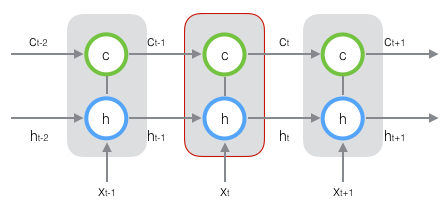
\includegraphics[width=0.8\textwidth]{lstm_2}
\caption{LSTM按时间维度展开图}
\label{fig:lstm_2}
\end{figure}
如图$\ref{fig:lstm}$为LSTM神经内部结构。上述表述的开关在LSTM中使用的门(gate)来实现的,门实际上就是一层全连接层,它的输入是一个向量,输出是一个0到1之间的实数向量。假设$W$是门的权重向量,$b$是偏置项,那么门可以表示为:
\begin{displaymath}
\begin{aligned}
g(x)=\sigma (W x+b)
\end{aligned}
\end{displaymath}
门的使用,就是用门的输出向量按元素乘以我们需要控制的那个向量。因为门的输出是0到1之间的实数向量,那么,当门输出为0时,任何向量与之相乘都会得到0向量,这就相当于啥都不能通过;输出为1时,任何向量与之相乘都不会有任何改变,这就相当于啥都可以通过。因为$\sigma$(也就是sigmoid函数)的值域是(0,1),所以门的状态都是半开半闭的。

LSTM用两个门来控制单元状态c的内容,一个是遗忘门(forget gate),它决定了上一时刻的单元状态$c_{t-1}$有多少保留到当前时刻;另一个是输入门(input gate),它决定了当前时刻网络的输入$x_{t}$有多少保存到单元状态。LSTM用输出门(output gate)来控制单元状态$c_{t}$有多少输出到LSTM的当前输出值$h_{t}$。

遗忘门:
\begin{equation}
\begin{aligned}
f_{t}=\sigma (\mathbf{W}_{f} \cdot [h_{t-1}, x_{t}]+b_{f})
\end{aligned}
\end{equation}

上式中,$\mathbf{W}_{f}$ 是遗忘门的权重矩阵,$[h_{t-1}, x_{t}]$表示把两个向量连接成一个更长的向量,$b_{f}$是遗忘门的偏置项,$\sigma$是sigmoid函数。

输入门:
\begin{equation}
\begin{aligned}
i_{t}=\sigma (\mathbf{W}_{i} \cdot [h_{t-1}, x_{t}]+b_{i})
\end{aligned}
\end{equation}
上式中,$\mathbf{W}_{i}$是输入门的权重矩阵,$b_{i}$是输入门的偏置项。

用于描述当前输入的单元状态$\tilde{c}_{t}$,它是根据上一次的输出和本次输入来计算的:
\begin{equation}
\begin{aligned}
\tilde{c}_{t}=\tanh (\mathbf{W}_{c} \cdot [h_{t-1}, x_{t}]+b_{c})
\end{aligned}
\end{equation}

计算当前时刻的单元状态$c_{t}$:
\begin{equation}
\begin{aligned}
c_{t}=f_{t} \circ c_{t-1} + i_{t} \circ \tilde{c}_{t}
\end{aligned}
\end{equation}
上式中,符号$\circ$表示按元素乘。它是由上一次的单元状态$c_{t-1}$按元素乘以遗忘门$f_{t}$,再用当前输入的单元状态$\tilde{c}_{t}$按元素乘以输入门$i_{t}$,再将两个积加和产生的。我们就把LSTM关于当前的记忆$\tilde{c}_{t}$和长期的记忆$c_{t-1}$组合在一起,形成了新的单元状态$c_{t}$。由于遗忘门的控制,它可以保存很久很久之前的信息,由于输入门的控制,它又可以避免当前无关紧要的内容进入记忆。

输出门,它控制了长期记忆对当前输出的影响:
\begin{equation}
\begin{aligned}
o_{t}=\sigma(W_{\sigma} \cdot [h_{t-1}, x_{t}]+b_{o})
\end{aligned}
\end{equation}

LSTM最中的输出,是由输出门和单元状态共同确定的:
\begin{equation}
\begin{aligned}
h_{t}=o_{t} \circ \tanh(c_{t})
\end{aligned}
\end{equation}

以上就是LSTM的前向计算。
\begin{figure}[htbp]
\centering
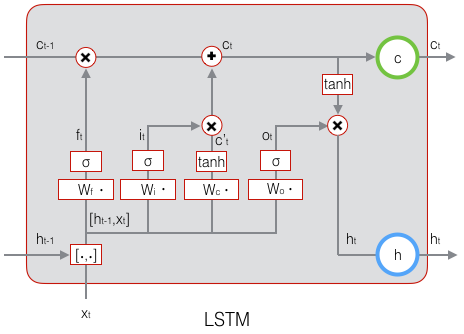
\includegraphics[width=0.8\textwidth]{lstm}
\caption{LSTM内部结构}
\label{fig:lstm}
\end{figure}

关于LSTM的训练过程仍然采用的反向传播算法,因为篇幅的限制具体计算过程不详细展开,主要包括以下三步:

(1)前向计算每个神经元的输出值,对于LSTM来说,即 $\mathbf{f}_{t}$、$\mathbf{i}_{t}$、$\mathbf{c}_{t}$、$\mathbf{o}_{t}$、$\mathbf{h}_{t}$五个向量的值。。

(2)反向计算每个神经元的误差项值。与循环神经网络一样,LSTM误差项的反向传播也是包括两个方向:一个是沿时间的反向传播,即从当前t时刻开始,计算每个时刻的误差项;一个是将误差项向上一层传播。

(3)根据相应的误差项,计算每个权重的梯度。


\subsection{一步混合模型}
% 就像第一节所描述的那样,因为强化学习考虑到了未来的回报,而且它的目标是直接优化长期奖赏,这与在直复营销场景中所期望的最大化客户ltv的目标是一致的。
基于RNN的深度强化学习模型(RL-RNN和RL-LSTM)在模型的的计算和训练上与DQN是类似的,但是因为循环神经网络通过对未来奖赏的长短时依赖性进行建模从而可以更好的处理序列中的部分可观测问题的原因,被广泛应用在序列问题的处理上\citep{bakker2002reinforcement,hausknecht2015deep,lin1993reinforcement,narasimhan2015language}。它们所设计的模型可以使用图$\ref{fig:rl_rnn}$表示。

在图$\ref{fig:rl_rnn}$中,$o_{t}$是观测值,$\tilde{h}_{t}$为RNN的隐藏状态,此处的当前隐藏状态是对其内部历史信息的概要总结。$Q(s,a)_{t}$是在时间$t$下采取行为$a$并且状态$s$为$\tilde{h}_{t}$的预测Q值。即Q网络是关于当前观测$o_{t}$和当前内部历史概要信息(隐藏层)$\tilde{h}_{t-1}$的函数,随着时间的推移,内部历史信息$\tilde{h}_{t}$将循环的更新,当Q网络学习完毕后,以贪婪的方式选择最优的行为。
\begin{figure}[htbp]
\centering
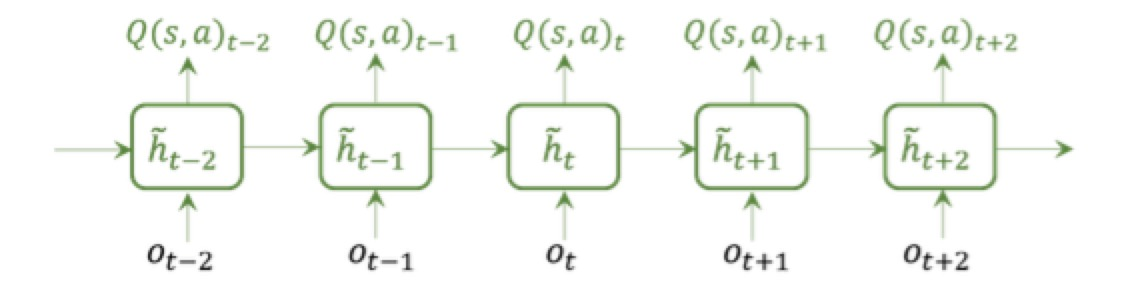
\includegraphics[width=1.0\textwidth]{rl_rnn}
\caption{RL-RNN框架}
\label{fig:rl_rnn}
\end{figure}

在RL-RNN模型中,因为RNN网络具有捕捉长期依赖性的强大能力,所以可以较好的估计Q函数。但是,在网络优化的过程中,RNN还需要可以很好的解决部分可观测的问题,那么如果要同时达到这两个目的,对于只有一个网络结构的RL-RNN来说是很难的。

所以,我们可以考虑具有两个网络的混合模型。可以使用强化学习模型,最大限度的获得长期回报,同时,可以对观测值和即刻奖赏的预测以训练优化监督学习模型,从而具有更好的推断和表示隐藏状态的能力。在这种混合方法中,使用监督学习来进行隐藏状态的表示学习,使用强化学习进行策略的学习,通过强化学习和监督学习的优势互补,可以使的这种混合模型达到很好的预测效果。另外,需要特别强调的是,这两个模型不能单独进行优化,而应该在监督学习了一个内部隐状态表示后就用强化学习模型最大化长期的奖赏。

使用以上混合模型的思想,我们可以得到基于rnn(lstm)和dqn的混合模型,即用rnn(lstm)进行监督模型的训练,使用dqn进行强化学习的训练,我可以将模型记为SL-RNN-RL-DQN(SL-LSTM-RL-DQN)。混合模型的网络结构如图$\ref{fig:rnn_dqn}$所示:
\begin{figure}[htbp]
\centering
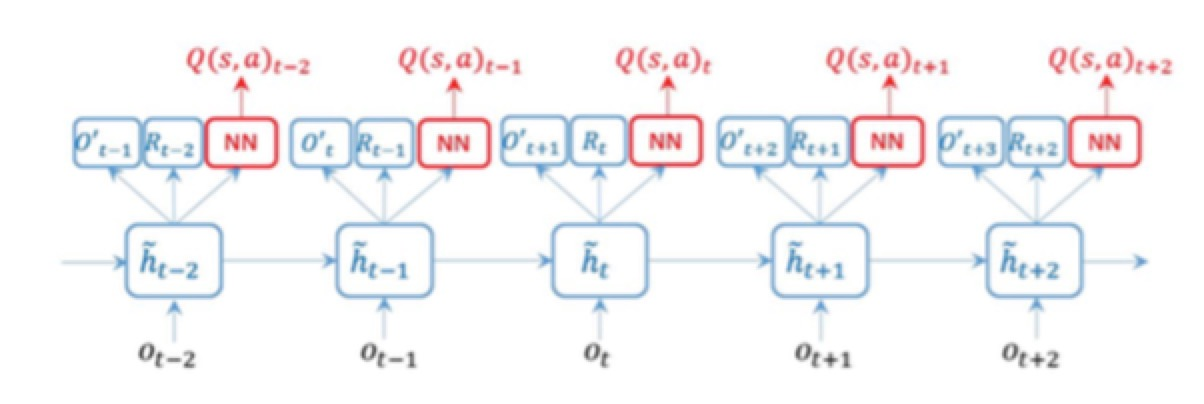
\includegraphics[width=1.0\textwidth]{rnn_dqn}
\caption{rnn-dqn框架}
\label{fig:rnn_dqn}
\end{figure}

在图$\ref{fig:rnn_dqn}$中,$o_{t}$是观测值,$h_{t}$是RNN的隐藏状态,$o_{t+1}^{'}$是$t+1$ 时刻的预测的观测值,$R_{t}$是预测的奖赏。$Q(s,a)_{t}$是t时刻预测的Q值,蓝色部分对应着RNN的监督学习部分,红色部分对应着DQN的学习部分。在混合模型中,DQN的输入是有监督的RNN模型。在训练阶段,我们使用联合训练的方法,首先我们在一个时刻从下一步的观测值和即时奖赏的信号中训练rnn(或者lstm)以学习隐藏状态的表示方法,然后,将学习到的隐藏状态作为DQN的输入,去学习近似最优策略的Q函数。以上这两个训练步骤在随机梯度下降迭代过程中交错进行。

因为在RNN-DQN学习的全部过程中,监督学习和强化学习模型按照上述训练方法依次进行学习,在学习过程中没有发生网络结构的变化,因此我们称之为一步混合模型,记为1-RNN-DQN。

由此,我们可以得到1-RNN-DQN模型的流程图以及损失函数的构造图。

\subsection{两步混合模型}
在上述的1-RNN-DQN模型中,先使用监督模型rnn进行隐藏状态的表示学习,再使用dqn进行策略的学习。在训练的过程中,监督信号将学习到的状态信息,反向传播到rnn或者lstm的头部,而强化学习只是将误差信号反向传播到rnn隐藏层,不参加rnn的训练。这种独立的训练方法虽然可以加快网络的训练速度,但是,因为两部分的误差信号是没有联系的,所以会造成这两部分网络的训练不平衡,从而影响最终的预测性能。这种不平衡性主要表现在1)rnn网络训练的不充分性影响了dqn的训练结果,从而造成了在rnn网络没有得到很好的隐状态表示时,但是dqn网络可能已经基于这种不好的表示而完成了较好的训练。2)即使两部分的网络都已经很好的完成了训练,但是这种割裂的误差传播仍然影响最终的表现。

基于以上的想法,我们提出了两步混合模型,记为2-RNN-DQN。在2-RNN-DQN中分为两个阶段,第一阶段按照2-RNN-DQN的方法进行训练,学习到两个网络的参数向量$\mathbf{\omega_{'}}$和$\mathbf{\omega_{''}}$,第二阶段将rnn网络的隐藏层和dqn网络的输入层连接起来,组成一个新的网络$[\mathbf{\omega_{'}},\mathbf{\omega_{''}}]$。新的网络的输入是观测值,输出是Q函数。具体学习过程是:将观测值输入到新的网络中,输出一个估计得Q值,然后利用误差学习更新整个网络的参数。

算法流程图如下。

\subsection{对照实验模型}

到目前为止,我们已经得到了DQN、RL-RNN、RL-lstm、1-SL-RNN+RL-dqn、1-SL-lstm+RL-dqn、2-SL-RNN+RL-dqn、2-SL-lstm+RL-dqn的模型的方法,作为对照组,我们提供了监督学习的训练方法。

在监督学习的模型中,我们的目标是从给定的到目前为止的交互历史中,预测可以导致更高的即刻奖赏的行为。在我们的实验中,我们使用原始奖赏信号作为目标进行回归预测。对于训练数据中的任意一个转移样本($o,a,r,o_{'}$),我们需要学习在给定观测o下奖赏r的回归曲线。我们主要考虑一下三个模型。

多层深度神经网络模型。该模型将交互历史分成单个的转移样本${(o_{t}, a_{t}, r_{t}, o_{t+1})}_{t=1,2,\cdots}$,基于($o_{t},a_{t}$)来学习预测$r_{t}$。这个模型使用$\hat{R}$来表示,在测试过程中,将目前的观测量$o$作为输入,通过奖赏的预测贪婪的选择行为:$\argmax_{a}\hat{R}(s,a)$。

RNN和LSTM可以从历史的交互中对长期依赖性进行建模。像图$\ref{fig:rnn_}$所示,$o_{t}$为观测值,$\tilde{h}_{t}$为rnn的内部状态,$R(s,a)_{t}$为在$t$时刻的预测的奖赏值,其中$s$是rnn的$\tilde{h}_{t}$。客户的交互历史不再像DNN那样被分解为单一的转移样本。在t时刻,这个模型使用观测值$o_{t}$,奖赏$r_{t}$以及目前的内部历史总结$\tilde{h}_{t-1}$来进行更新,并且在rnn中循环的保持这种更新方式。在测试阶段,模型基于当前的观测值和当前的内部历史概要信息来选择行为。lstm的过程和rnn过程类似。
\begin{figure}[htbp]
\centering
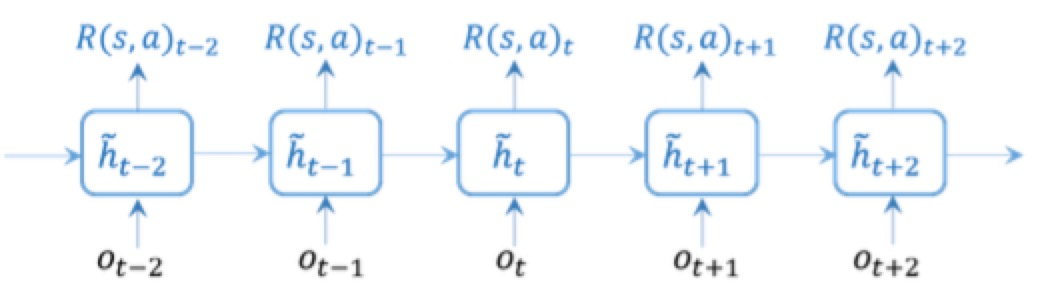
\includegraphics[width=1.0\textwidth]{rnn_}
\caption{rnn训练展开图}
\label{fig:rnn_}
\end{figure}

\section{本章小结}